\begin{figure}[H]
	\centering
	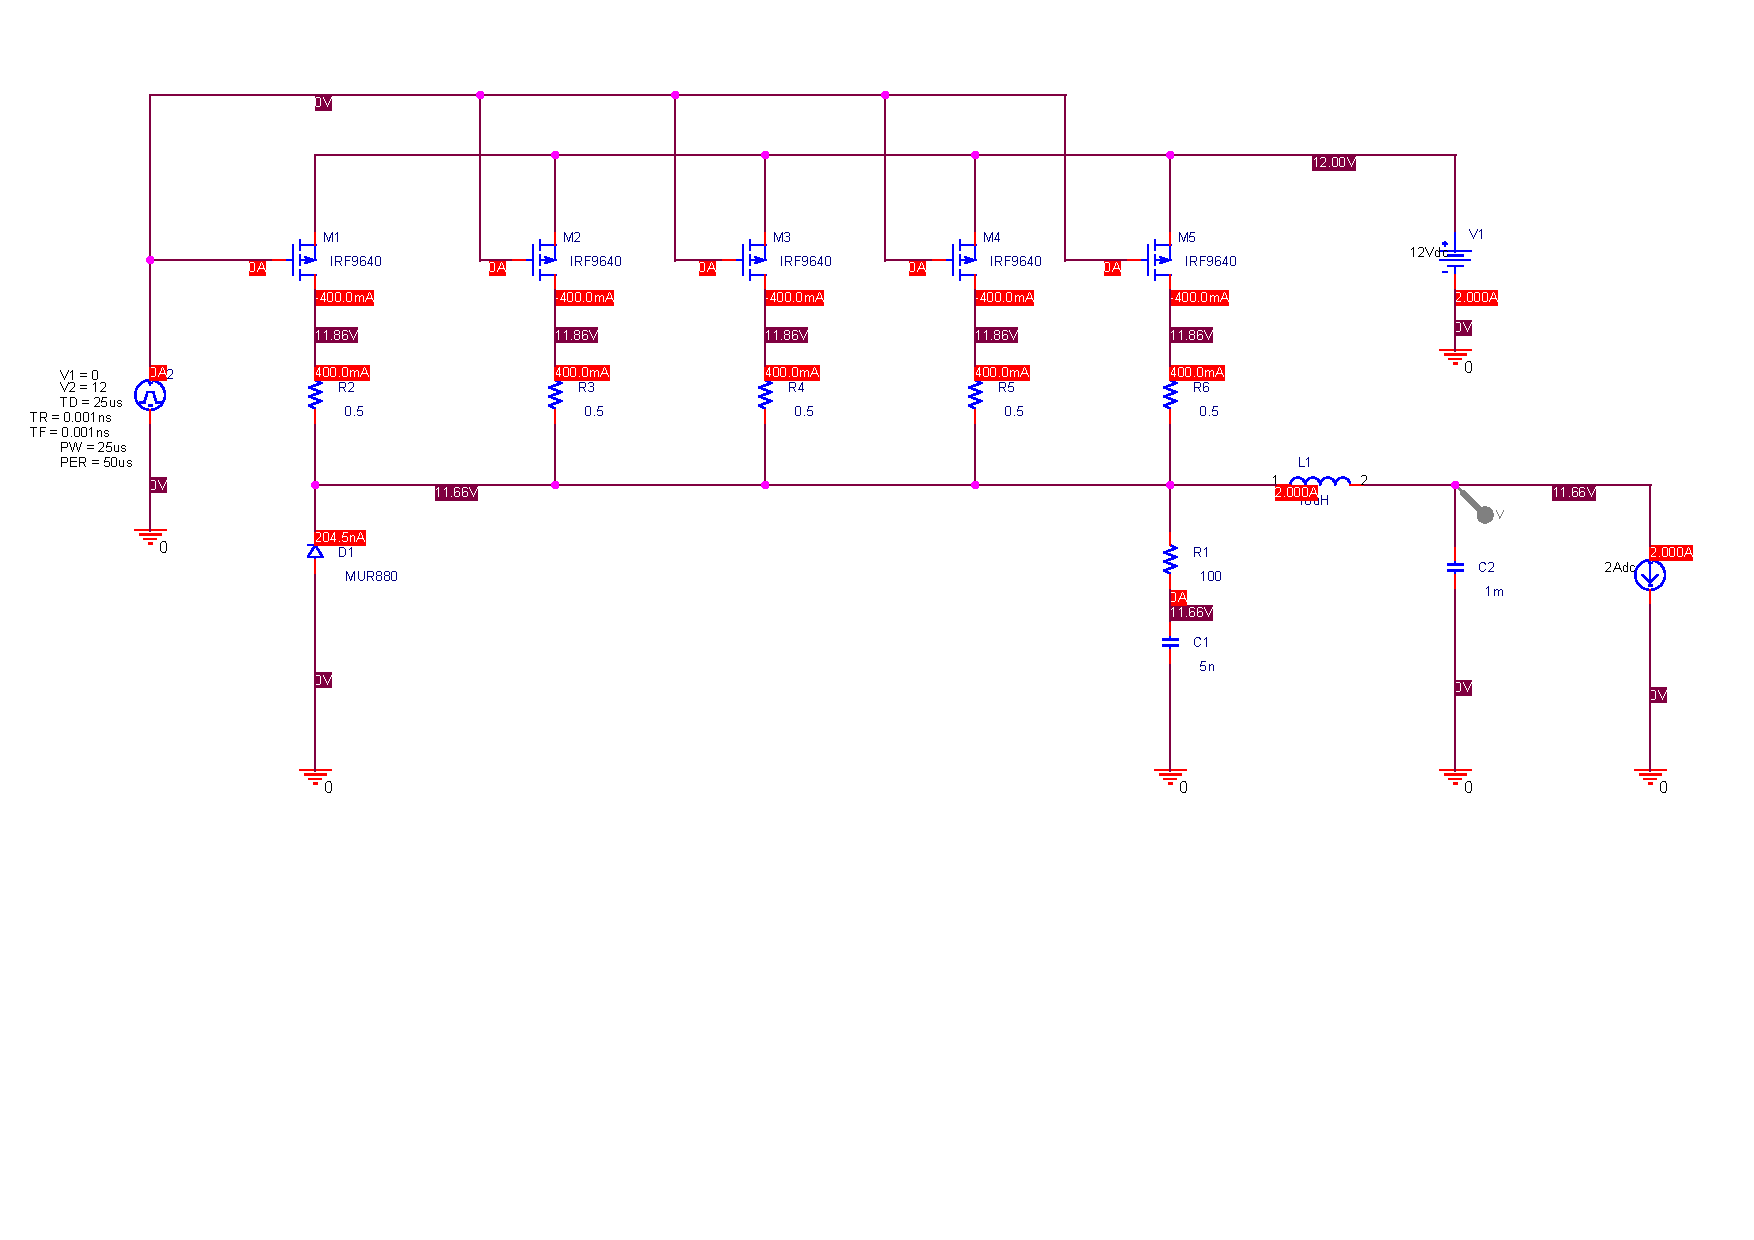
\includegraphics[scale=0.4]{Figuras/ej1_esq_sim.pdf}
	\caption{Simulación en \textit{PSpice}}
	\label{fig:ej1_esq_sim}
\end{figure}

Se simuló el circuito según la Figura \ref{fig:ej1_esq_sim}, obteniéndose una tensión de salida de \SI{9}{\volt} luego del transitorio. (ver Figura \ref{fig:sim_ej1_vo}).

\begin{figure}[H]
	\centering
	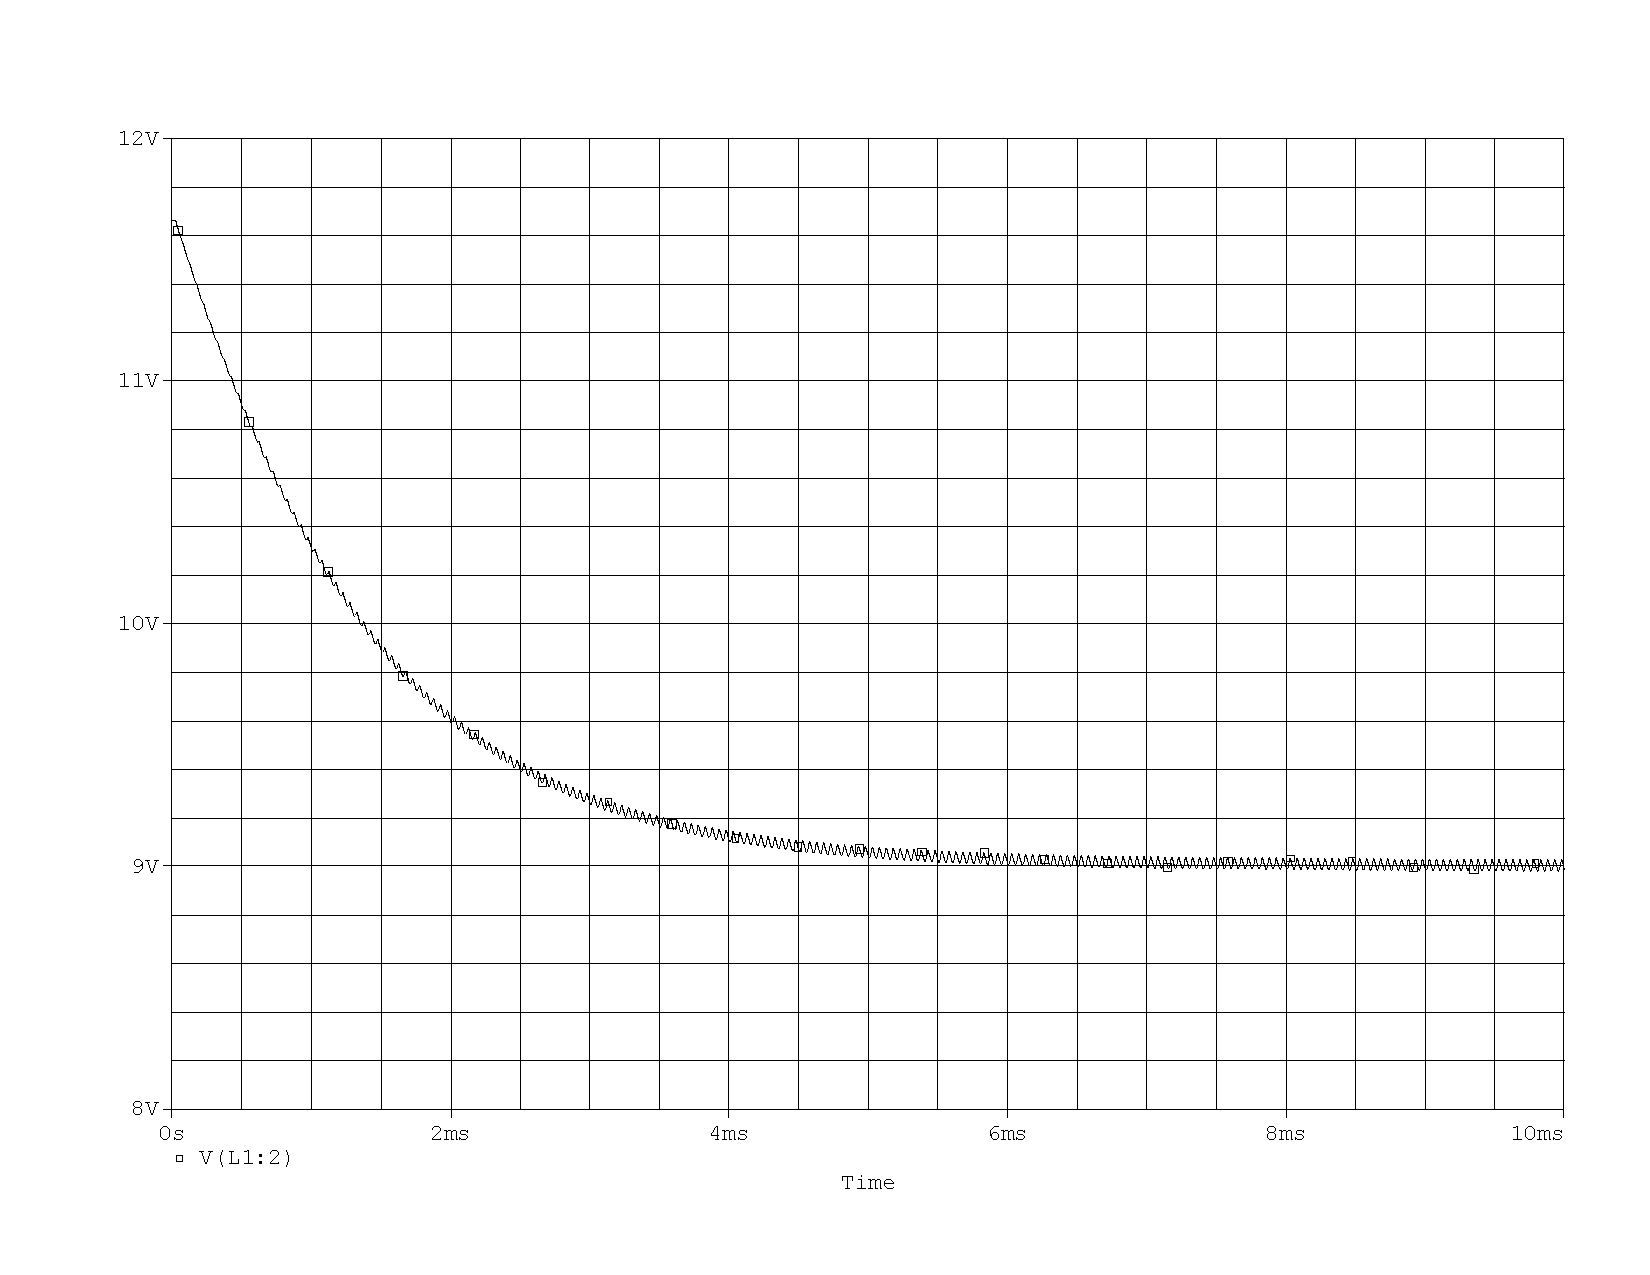
\includegraphics[scale=0.4]{Figuras/ej1_vo.pdf}
	\caption{Tensión de salida.}
	\label{fig:sim_ej1_vo}
\end{figure}

\begin{figure}[H]
	\centering
	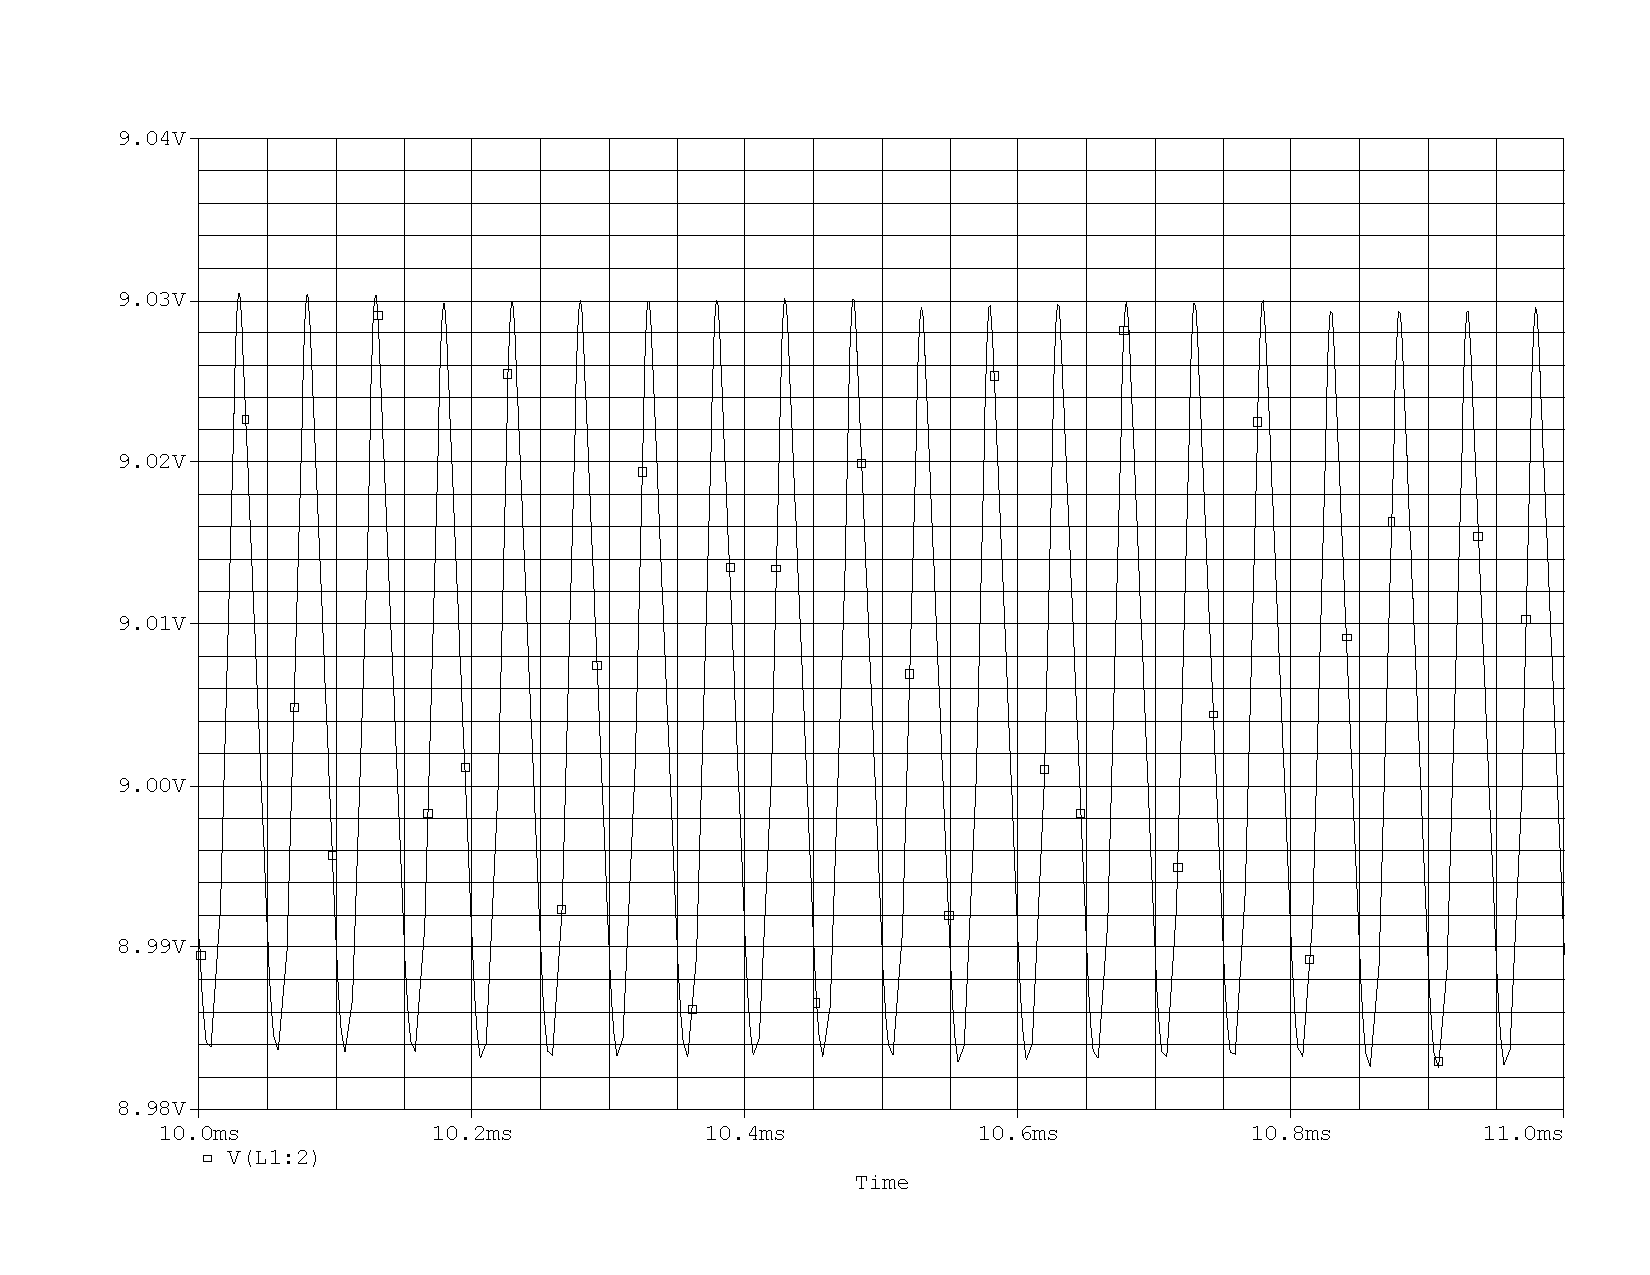
\includegraphics[scale=0.4]{Figuras/ej1_vo_zoom.pdf}
	\caption{Tensión de salida.}
	\label{fig:sim_ej1_vo_zoom}
\end{figure}

Una ampliación de la tensión de salida se observa en el Gráfico \ref{fig:sim_ej1_vo_zoom}, siendo el valor de rizado \eqref{ec:riz1}.

\begin{equation}
	\centering
	\Delta V_o = \SI{9.0299}{\volt} - \SI{8.9834}{\volt} = \boxed{\SI{46.5}{\milli\volt}}
	\label{ec:riz1}
\end{equation}

\begin{figure}[H]
	\centering
	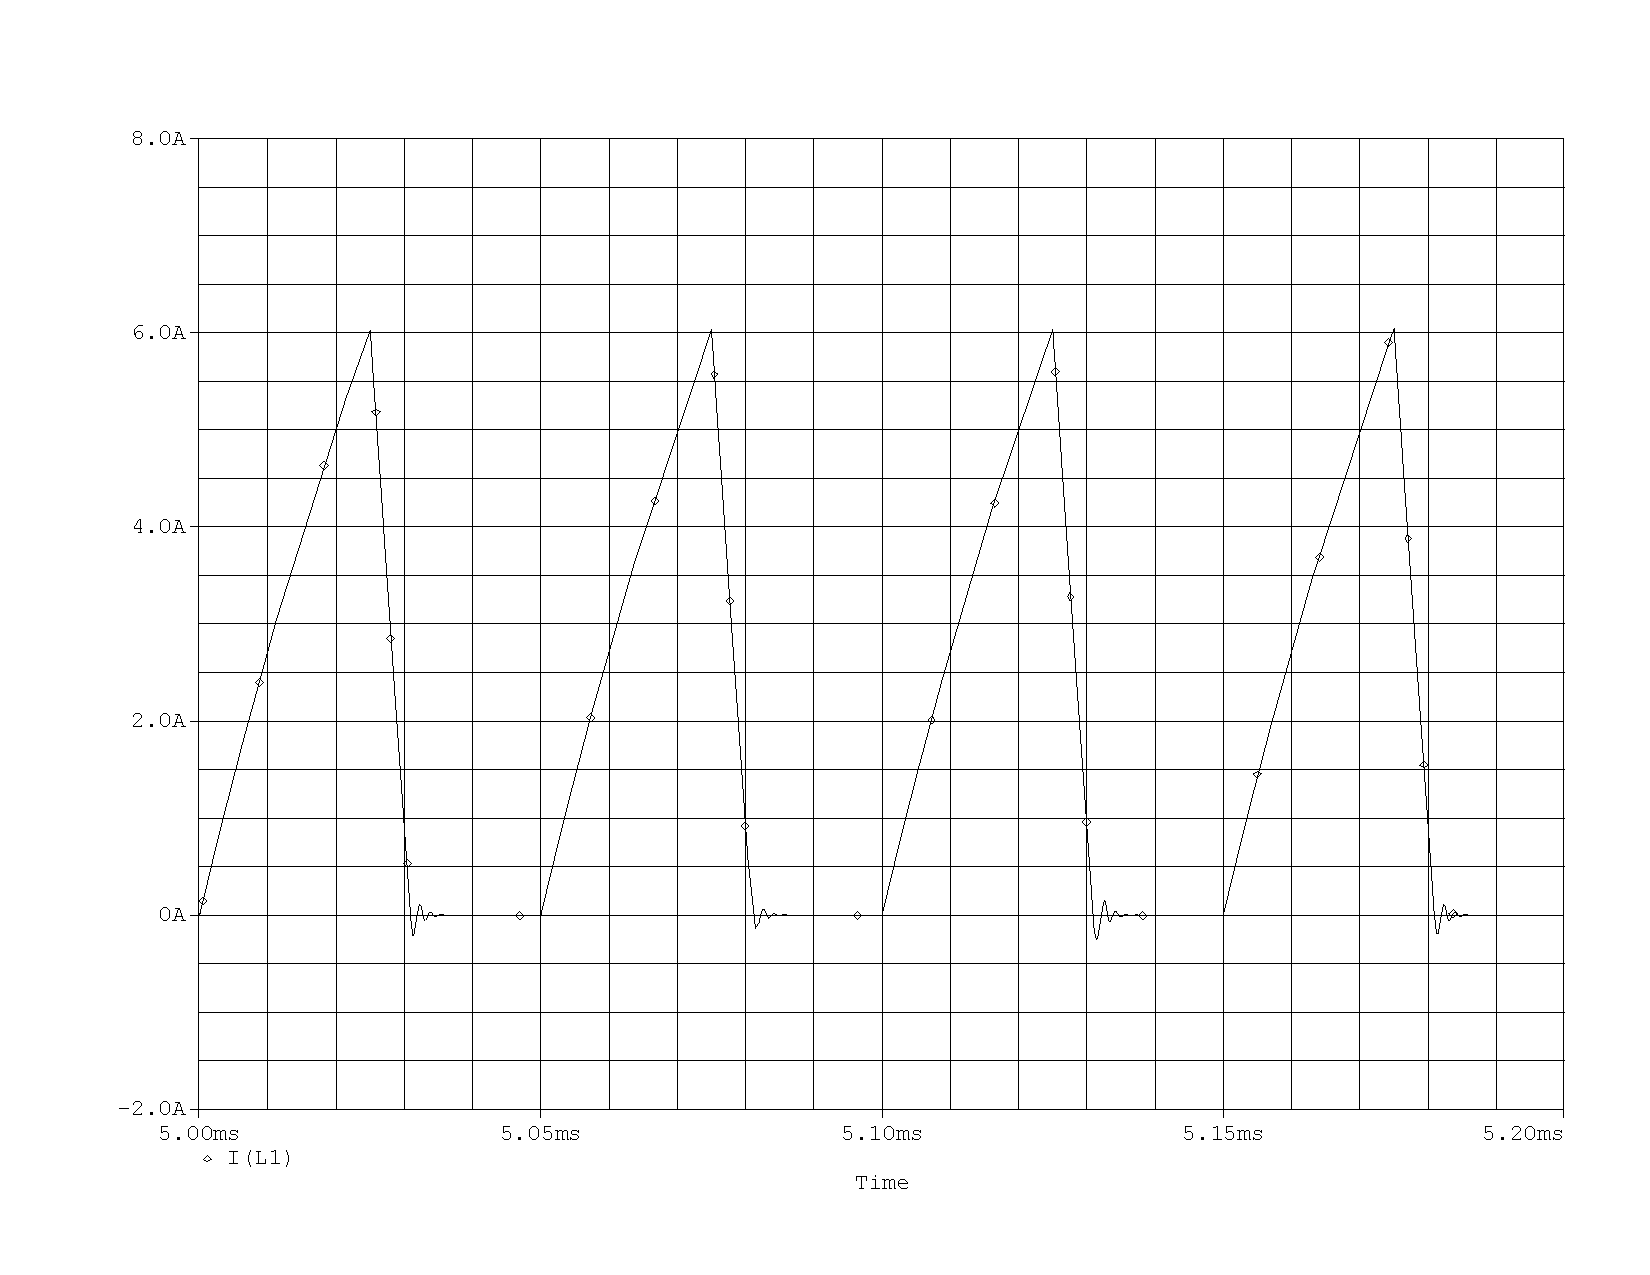
\includegraphics[scale=0.4]{Figuras/ej1_I(L1).pdf}
	\caption{Corriente en el inductor.}
	\label{fig:sim_ej1_il}
\end{figure}

